\documentclass[aspectratio=169]{beamer}
\usetheme{Madrid}

\usepackage{graphicx}
\usepackage[utf8]{inputenc}
\usepackage{hyperref}
\usepackage{listings}
\usepackage{xcolor}
\usepackage{subfig}

%\setbeamertemplate{footline}[frame number]

\begin{document}

\title{Introduction to Neural Networks}  
\subtitle{Transposed convolution} 
\author[J.I. Vasquez]{\textbf{Juan Irving Vásquez} \\jivg.org}
\date{\today \copyright}
\institute[jivg.org]{Centro de Innovación y Desarrollo Tecnológico en Cómputo \\ Instituto Politécnico Nacional}
% logo of my university
\titlegraphic{
\includegraphics[height=1.2cm]{ipn-cidetec.png}\hspace{0.1cm}
\includegraphics[height=1.2cm]{escudoESCOM}}
{ 	%\usebackgroundtemplate{
\includegraphics[width=1\paperwidth]{markus-winkler-afW1hht0NSs-unsplash}}%
\frame{\titlepage}
}


\begin{frame}
	\frametitle{Motivation}
	\framesubtitle{Reduction of the feature map}
\begin{figure}
	\centering
	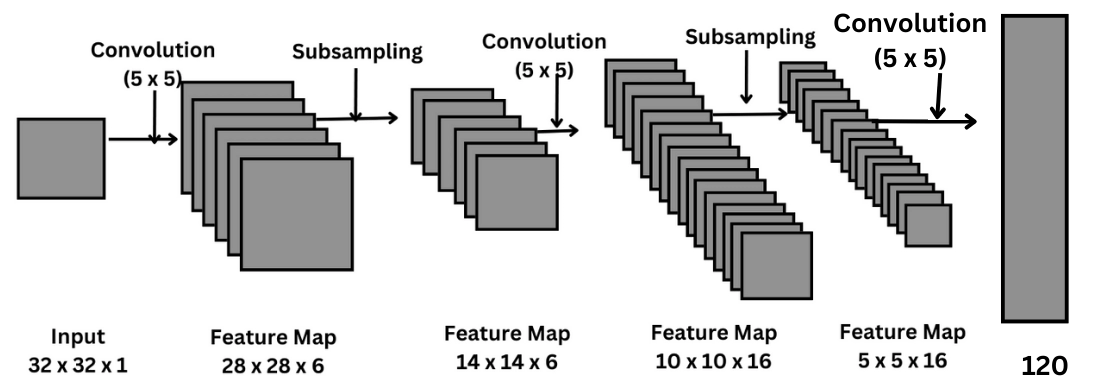
\includegraphics[height=0.5\textheight]{lenet_cnn}
	\caption{Convolutional part of LeNet5}
	\label{fig:lenetcnn}
\end{figure}
\end{frame}


\begin{frame}
	\frametitle{Inverse convolution}
	\begin{itemize}
		\item Given that
		$$ G = I \star K $$
		\item Is this possible?
		$$ I = G \star K^{-1}  $$
		\pause		
		\item In theory, but it is not practical, it involves the computation of a inverse matrix.
		\item Therefore we will apply a transposed convolution instead.
	\end{itemize}
\end{frame}


\begin{frame}
	\frametitle{Information loss}
	\begin{center}
		
\includegraphics[height=0.7\textheight]{bb}
		\pause
		\hspace{20pt}
		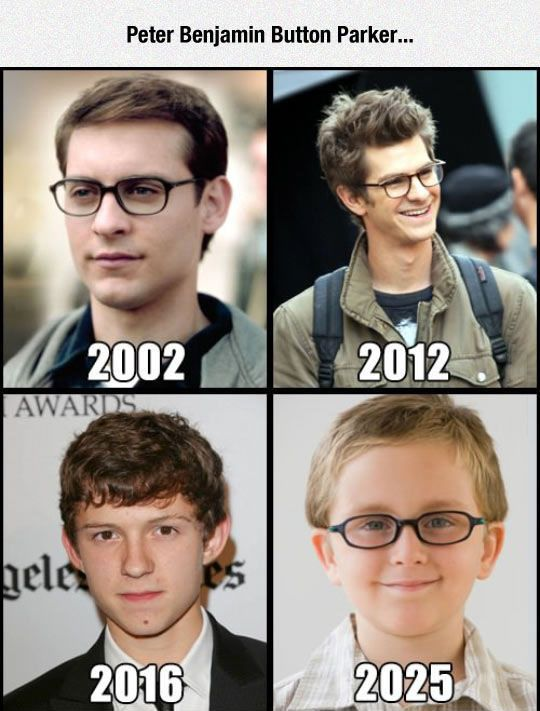
\includegraphics[height=0.7\textheight]{pp}
	\end{center}
\end{frame}


\begin{frame}
	\frametitle{Transposed convolution}
	\begin{itemize}
		\item Reverse the dimension of the convolution operation, upsampling
		$$ G = I \star K $$
		$$ T = G \star \star W $$
		$$ |T| = |I| $$
		$$  T \approx I $$
		
		\item Transposed convolution doesn’t reverse the standard convolution by values
	\end{itemize}
	
\begin{center}
	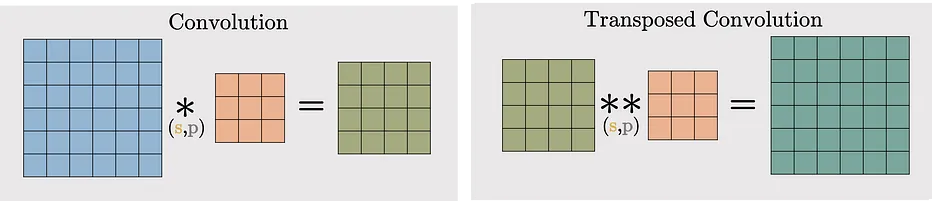
\includegraphics[height=0.3\textheight]{tranpconv}
\end{center}
\end{frame}




\begin{frame}
	\frametitle{Transposed convolution}
	\begin{center}
		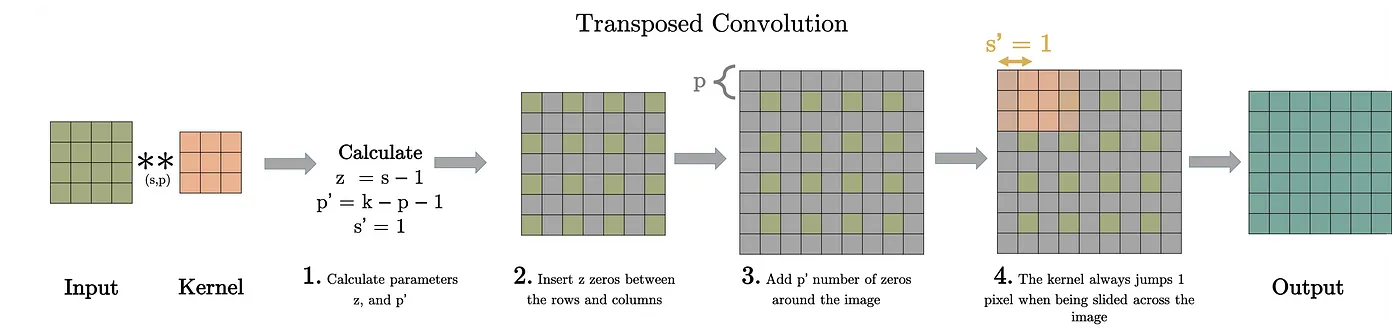
\includegraphics[height=0.35\textheight]{tconvanim}
	\end{center}

	\begin{enumerate}
		\item Calculate parameters $z$ and $p'$:
		\begin{equation}
			z = s - 1 
		\end{equation}
		\begin{equation}
			p' = k - p - 1
		\end{equation}
		\item Between each row and columns of the input, $G$, insert $z$ number of zeros. 
		\item Pad the modified input image with $p’$ number of zeros
		\item Perform a convolution, $G\star W$, with stride $s' = 1$
	\end{enumerate}

\end{frame}



\begin{frame}
\frametitle{References}
\begin{itemize}
	\item Dumoulin, Vincent, and Francesco Visin. "A guide to convolution arithmetic for deep learning." arXiv preprint arXiv:1603.07285 (2016).
	\item Aqeel Anwar, What is Transposed Convolutional Layer?, https://towardsdatascience.com/what-is-transposed-convolutional-layer, Consultado: Abril 2023.
\end{itemize}
\end{frame}

\end{document}